\documentclass{article}

\usepackage[latin1]{inputenc}
\usepackage{tikz}
\usetikzlibrary{calc}
\usepackage{tkz-euclide}
\tikzset{line/.style={draw, thick, -latex'}}
%\usetikzlibrary{shapes,arrows}
\begin{document}
\pagestyle{empty}


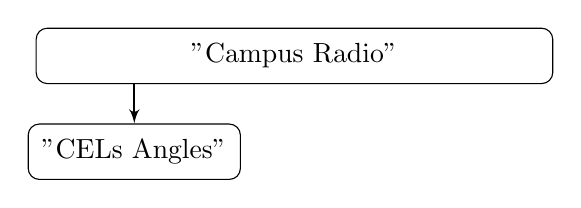
\begin{tikzpicture}[node distance = 1cm, auto]
\tikzstyle{block} = [rectangle, rounded corners, draw, text width=6em, text centered, minimum height=2em]
\tikzstyle{rect} = [rectangle, draw, text width=5.9em, text centered, minimum height=2em]
\tikzstyle{input} = [rectangle, text width=2em, align=right, minimum height=2em]

\node [block, text width=18em](ensemble){"Campus Radio"};
\node [block, below=0.5cm of ensemble.190, anchor=north, text width=7em](sender1){"CELs Angles"};


\path [line] (ensemble.190) -- (sender1.north);


\end{tikzpicture}
\end{document}